\documentclass[senior]{IPSstyle}


\Year{2020}
\Month{July}
\Author{44181528-1}

\Title{DualBox}

\Advisor{Professor YOSHIE}

\usepackage{amssymb,amsmath}

\usepackage{array}
\usepackage{mathptmx}
\usepackage{helvet}
\usepackage{courier}
\usepackage{type1cm}

\usepackage{makeidx}
\usepackage{graphicx,subfigure}
\usepackage{multicol}
\usepackage{multirow}
\usepackage[bottom]{footmisc}

\usepackage{mathrsfs}
\usepackage{amssymb,amsmath}
\usepackage{amsfonts}
\usepackage{color}
\usepackage{CJKutf8}
\usepackage{smartdiagram}
\usepackage{caption}

\usepackage{listings}
\usepackage{algorithm,algorithmicx,algpseudocode}
\usepackage[toc,page,title,titletoc,header]{appendix}

\DeclareMathOperator*{\otherwise}{otherwise}

\renewcommand{\algorithmicrequire}{\textbf{Input:}}
\renewcommand{\algorithmicensure}{\textbf{Output:}}

\Abstract{

    Thank you.
}

\begin{document}
\makepreliminarypages
\singlespace
\frontmatter
\tableofcontents
\listoffigures
\listoftables
\mainmatter
\clearemptydoublepage
\setlength{\baselineskip}{23.0pt}

%%%%%%%%%%%%%%%%%%%%%%%%%%%%%%%%%%%%%%%%%%%%%%%%%%%%%%%%%%%%%%Chapter 1
\chapter{Introduction} 
%%%%%%%%%%%%%%%%%%%%%%%%%%%%%%%%%%%%%%%%%%%%%%%%%%%%%%%%%%%%%%Chapter 1


\begin{figure}[t]
    \begin{center}
    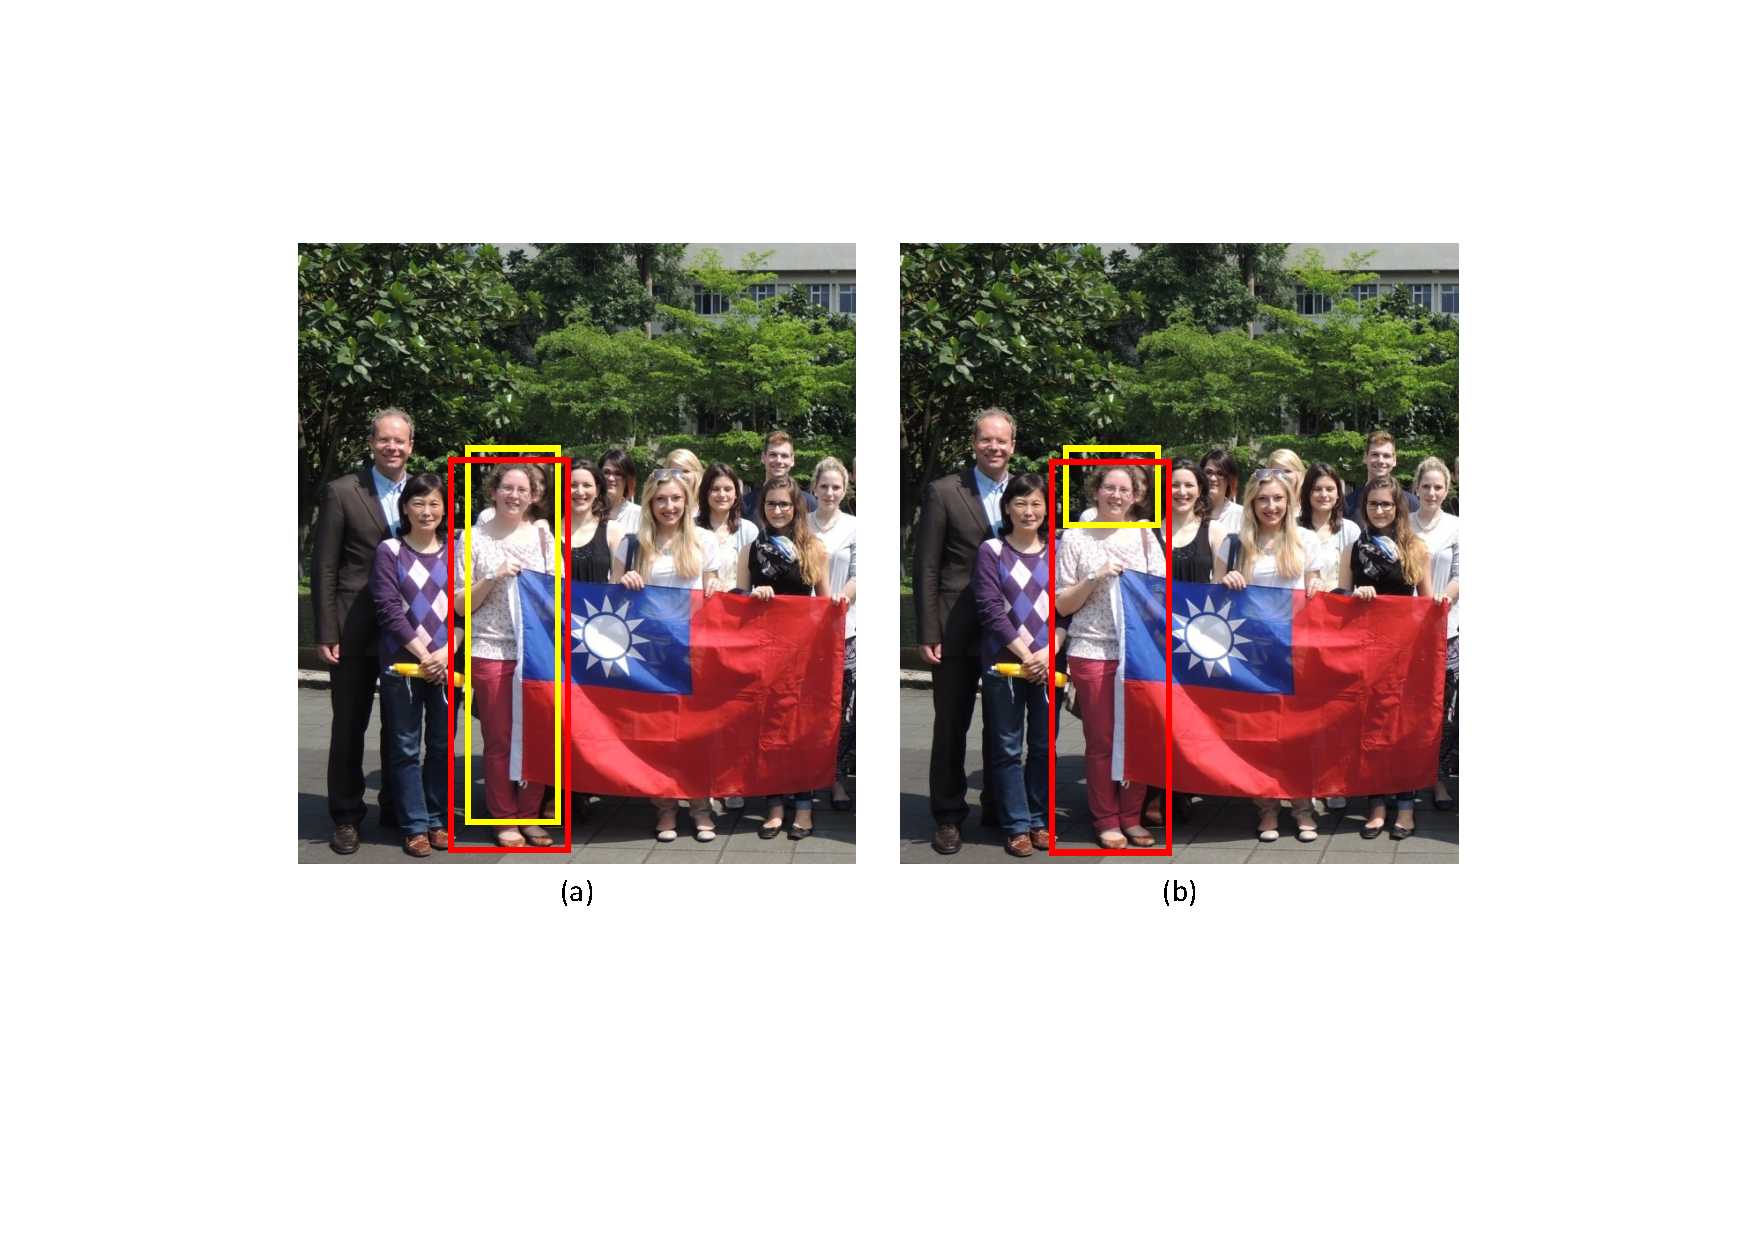
\includegraphics[width=0.97\linewidth]{images/start.pdf}
    \end{center}
\vspace{-0.3cm}
    \caption{ }
    \label{fintro}
    \vspace{-0.3cm}
\end{figure} 



%--------------------------------------------------------------------------
\section{Related works}
%--------------------------------------------------------------------------

%--------------------------------------------------------------------------
\subsection{Generic Object Detection}
%--------------------------------------------------------------------------


\bibliographystyle{plain}
\bibliography{references}
\end{document}